
\section{Injektivität, Surjektivität und Bijektivität von Abbildungen}

\subsection{Injektivität von Abbildungen}

\textbf{Definition (injektiv):}

Eine Abbildung $f:\mathbb{D}_f\longrightarrow\mathbb{W}_f$
heißt injektiv, wenn aus $f(x_1)=f(x_2)$ stets
$x_1=x_2$ folgt. Mathematisch gilt:
\[
\forall x_1,x_2\in\mathbb{D}_f:\quad
f(x_1)=f(x_2)\ \Longrightarrow\ x_1=x_2.
\]

\textbf{Beispiel:} $f_2:\mathbb{R}\longrightarrow[0,\infty[$,
$f_2(x)=x^2$.

Zeige, dass $f_2$ nicht injektiv ist.
\begin{quote}
Für die verschiedenen Argumente $x_1=-1$ und $x_2=1$ gilt
\[
f_2(-1)=(-1)^2=1=(1)^2=f_2(1).
\]
Also gilt $x_1\neq x_2$, obwohl $f_2(x_1)=f_2(x_2)$.
Damit ist die Injektivitätsbedingung verletzt;
$f_2$ ist nicht injektiv.
\end{quote}

\begin{center}
	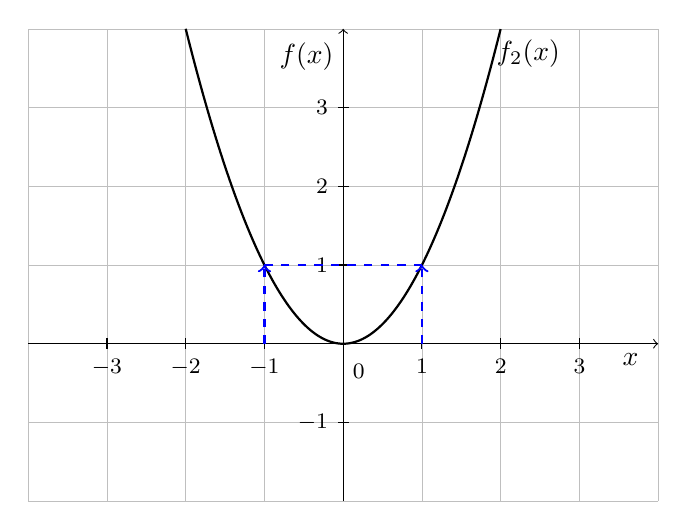
\begin{tikzpicture}
		
		% Gitternetzlinien
		\draw[xstep=1cm, ystep=1cm, very thin, color=lightgray] (-4,4) grid (4,-2);
		% x-Achse
		\draw[->] (-4,0) -- (4,0) node[below,xshift=-1em] {$x$}; 
		%Zahlen auf x-Achse
		\foreach \x in {-3,...,-1}
		\draw[shift={(\x,0)},color=black] (0pt,2pt) -- (0pt,-2pt) node[below] {\footnotesize $\x$};
		\foreach \x in {1,...,3}
		\draw[shift={(\x,0)},color=black] (0pt,2pt) -- (0pt,-2pt) node[below] {\footnotesize $\x$};
		% y-Achse 
		\draw[->] (0,-2) -- (0,4) node[left,yshift=-1em] {$f(x)$};%node[above left]
		%Zahlen auf y-Achse
		\foreach \y in {-1,...,-1}
		\draw[shift={(0,\y)},color=black] (2pt,0pt) -- (-2pt,0pt) node[left] {\footnotesize $\y$};
		\foreach \y in {1,...,3}
		\draw[shift={(0,\y)},color=black] (2pt,0pt) -- (-2pt,0pt) node[left] {\footnotesize $\y$};
		%Ursprung
		\draw[color=black] (0pt,-10pt) node[right] {\footnotesize $0$};
		
		
		
		\draw[thick,color=black] plot[samples=200, domain=-2:2] 
		(\x,{\x*\x}) node[below, xshift=1em]{$f_2(x)$};
		
		\draw[color=blue,thick,dashed] (-1,1) -- (1,1);
		\draw[->,color=blue,thick,dashed] (-1,0) -- (-1,1);
		\draw[->,color=blue,thick,dashed] (1,0) -- (1,1);
		
	\end{tikzpicture}\\
\end{center}
\newpage
\noindent
\textbullet \;\; Die Einschränkung $f_2|_{[0,\infty[}$ ist injektiv, da $x^2$ auf $[0,\infty[$ streng monoton wächst.
\begin{center}
	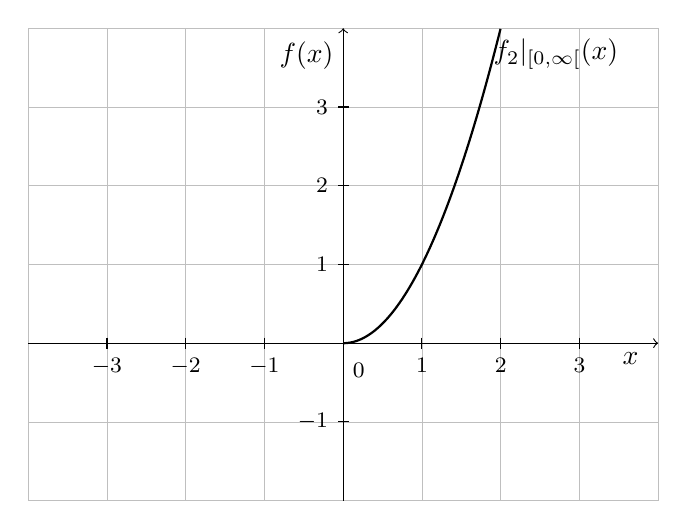
\begin{tikzpicture}
		
		% Gitternetzlinien
		\draw[xstep=1cm, ystep=1cm, very thin, color=lightgray] (-4,4) grid (4,-2);
		% x-Achse
		\draw[->] (-4,0) -- (4,0) node[below,xshift=-1em] {$x$}; 
		%Zahlen auf x-Achse
		\foreach \x in {-3,...,-1}
		\draw[shift={(\x,0)},color=black] (0pt,2pt) -- (0pt,-2pt) node[below] {\footnotesize $\x$};
		\foreach \x in {1,...,3}
		\draw[shift={(\x,0)},color=black] (0pt,2pt) -- (0pt,-2pt) node[below] {\footnotesize $\x$};
		% y-Achse 
		\draw[->] (0,-2) -- (0,4) node[left,yshift=-1em] {$f(x)$};%node[above left]
		%Zahlen auf y-Achse
		\foreach \y in {-1,...,-1}
		\draw[shift={(0,\y)},color=black] (2pt,0pt) -- (-2pt,0pt) node[left] {\footnotesize $\y$};
		\foreach \y in {1,...,3}
		\draw[shift={(0,\y)},color=black] (2pt,0pt) -- (-2pt,0pt) node[left] {\footnotesize $\y$};
		%Ursprung
		\draw[color=black] (0pt,-10pt) node[right] {\footnotesize $0$};
		
		
		
		\draw[thick,color=black] plot[samples=200, domain=0:2] 
		(\x,{\x*\x}) node[below, xshift=2em]{$f_2|_{[0,\infty[}(x)$};
		
		
		
	\end{tikzpicture}\\
\end{center}
\begin{quote}
	Merke: Die Injektivität hängt stark vom $ \mathbb{D}_f$ ab.
\end{quote}
\newpage
\noindent

Beispiel: $f:\mathbb{R}\rightarrow\mathbb{R}$ mit $f(x)=2$.
\begin{center}
	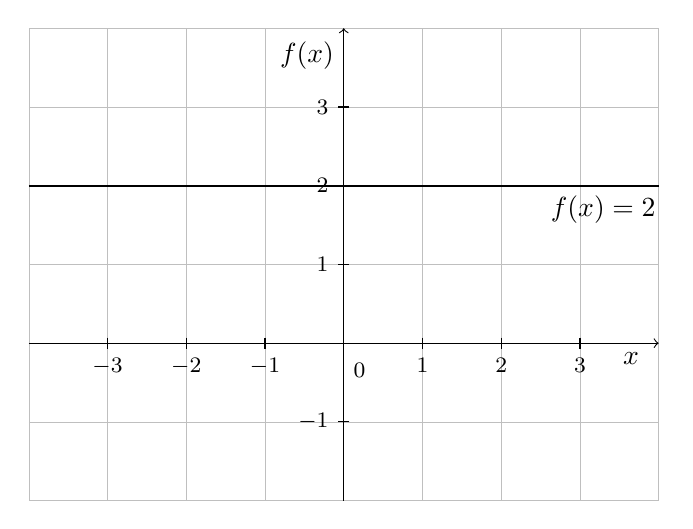
\begin{tikzpicture}
		
		% Gitternetzlinien
		\draw[xstep=1cm, ystep=1cm, very thin, color=lightgray] (-4,4) grid (4,-2);
		% x-Achse
		\draw[->] (-4,0) -- (4,0) node[below,xshift=-1em] {$x$}; 
		%Zahlen auf x-Achse
		\foreach \x in {-3,...,-1}
		\draw[shift={(\x,0)},color=black] (0pt,2pt) -- (0pt,-2pt) node[below] {\footnotesize $\x$};
		\foreach \x in {1,...,3}
		\draw[shift={(\x,0)},color=black] (0pt,2pt) -- (0pt,-2pt) node[below] {\footnotesize $\x$};
		% y-Achse 
		\draw[->] (0,-2) -- (0,4) node[left,yshift=-1em] {$f(x)$};%node[above left]
		%Zahlen auf y-Achse
		\foreach \y in {-1,...,-1}
		\draw[shift={(0,\y)},color=black] (2pt,0pt) -- (-2pt,0pt) node[left] {\footnotesize $\y$};
		\foreach \y in {1,...,3}
		\draw[shift={(0,\y)},color=black] (2pt,0pt) -- (-2pt,0pt) node[left] {\footnotesize $\y$};
		%Ursprung
		\draw[color=black] (0pt,-10pt) node[right] {\footnotesize $0$};
		
		
		
		\draw[thick,color=black] plot[samples=200, domain=-4:4] 
		(\x,{2}) node[below, xshift=-2em]{$f(x)=2$};
		
		
		
	\end{tikzpicture}\\
\end{center}
Diese Funktion ist nicht injektiv: Beispielsweise gilt $f(0)=f(1)=2$ bei $0\neq 1$.\vspace*{2mm}
\\
Beispiel: $f(x)=3\sin(x)+1$\\
\begin{center}
	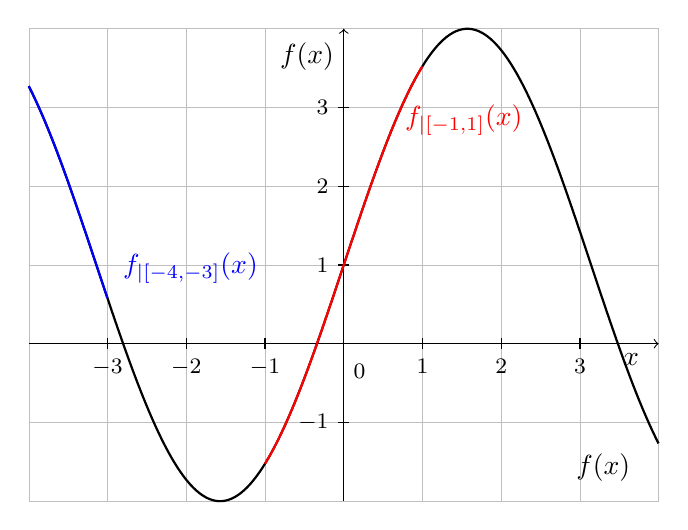
\begin{tikzpicture}
		
		% Gitternetzlinien
		\draw[xstep=1cm, ystep=1cm, very thin, color=lightgray] (-4,4) grid (4,-2);
		% x-Achse
		\draw[->] (-4,0) -- (4,0) node[below,xshift=-1em] {$x$}; 
		%Zahlen auf x-Achse
		\foreach \x in {-3,...,-1}
		\draw[shift={(\x,0)},color=black] (0pt,2pt) -- (0pt,-2pt) node[below] {\footnotesize $\x$};
		\foreach \x in {1,...,3}
		\draw[shift={(\x,0)},color=black] (0pt,2pt) -- (0pt,-2pt) node[below] {\footnotesize $\x$};
		% y-Achse 
		\draw[->] (0,-2) -- (0,4) node[left,yshift=-1em] {$f(x)$};%node[above left]
		%Zahlen auf y-Achse
		\foreach \y in {-1,...,-1}
		\draw[shift={(0,\y)},color=black] (2pt,0pt) -- (-2pt,0pt) node[left] {\footnotesize $\y$};
		\foreach \y in {1,...,3}
		\draw[shift={(0,\y)},color=black] (2pt,0pt) -- (-2pt,0pt) node[left] {\footnotesize $\y$};
		%Ursprung
		\draw[color=black] (0pt,-10pt) node[right] {\footnotesize $0$};
		
		
		
		\draw[thick,color=black] plot[samples=200, domain=-4:4] 
		(\x,{3*sin(\x r)+1}) node[below, xshift=-2em]{$f(x)$};
		
		\draw[thick,color=blue] plot[samples=200, domain=-4:-3] 
		(\x,{3*sin(\x r)+1}) node[below, xshift=3em,yshift=2em]{$f_{|[-4,-3]}(x)$};
		\draw[thick,color=red] plot[samples=200, domain=-1:1] 
		(\x,{3*sin(\x r )+1}) node[below, xshift=1.5em,yshift=-1em]{$f_{|[-1,1]}(x)$};
		
	\end{tikzpicture}\\
\end{center}
Die Funktion $f:\mathbb{R}\rightarrow\mathbb{R}$ mit $f(x)=3\sin(x)+1$ ist nicht injektiv, da sie periodisch ist. Auf den Intervallen $[-4,-3]$ und $[-1,1]$ ist sie dagegen jeweils streng monoton und daher injektiv.
\subsection{Surjektivität und Bijektivität von Abbildungen}

\textbf{Definition (surjektiv):}\\
Eine Abbildung
$f:\mathbb{D}_f\rightarrow\mathbb{W}_f$
heißt surjektiv, wenn zu jedem Element
$y$ der Zielmenge mindestens ein Element
$x$ des Definitionsbereichs existiert,
sodass $f(x)=y$ gilt.

Mathematisch:

\begin{align*}
	\forall y\in\mathbb{W}_f\;
	\exists x\in\mathbb{D}_f:
	\quad f(x)=y
\end{align*}




Beispiel:\\
\textbullet $\;\;f_2:\mathbb{R}\longmapsto\mathbb{R}$ mit $x\longmapsto x^2$\\
\begin{quote}
	Für $y=-1$ existiert kein $x$ mit $x^2=y=-1$\\
	$f_2$ ist nicht surjektiv.\vspace*{2mm}\\
\end{quote}
\pagebreak
\textbullet$\;\;\widetilde{f}_2: \mathbb{R}\longmapsto [0,\infty[$ mit $x\longmapsto x^2$\\
\begin{quote}
	Zum Nachweis der Surjektivität betrachten wir ein beliebiges Element $y$ der Zielmenge und suchen ein $x$ mit $\widetilde{f}_2(x)=y$.
	
	Sei $y\in [0,\infty[$ und wähle $ x=\sqrt{y} $\\
	$\widetilde{f}_2(\sqrt{y})=(\sqrt{y})^2=y$. Somit ist $\widetilde{f}_2$ surjektiv.
	
\end{quote}

\begin{center}
	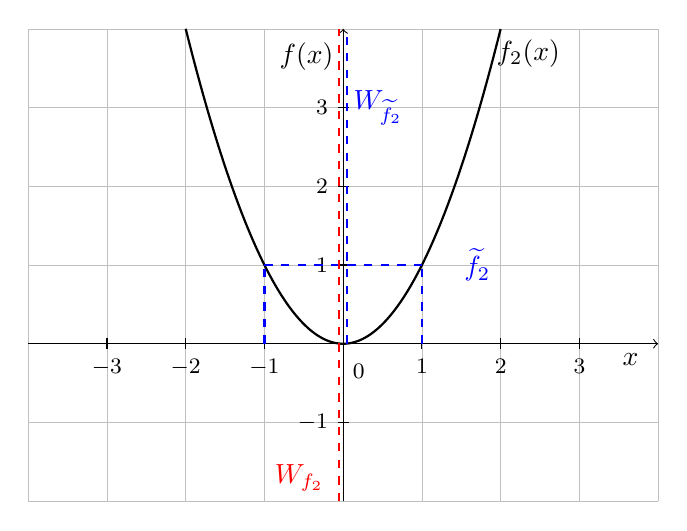
\begin{tikzpicture}
		
		% Gitternetzlinien
		\draw[xstep=1cm, ystep=1cm, very thin, color=lightgray] (-4,4) grid (4,-2);
		% x-Achse
		\draw[->] (-4,0) -- (4,0) node[below,xshift=-1em] {$x$}; 
		%Zahlen auf x-Achse
		\foreach \x in {-3,...,-1}
		\draw[shift={(\x,0)},color=black] (0pt,2pt) -- (0pt,-2pt) node[below] {\footnotesize $\x$};
		\foreach \x in {1,...,3}
		\draw[shift={(\x,0)},color=black] (0pt,2pt) -- (0pt,-2pt) node[below] {\footnotesize $\x$};
		% y-Achse 
		\draw[->] (0,-2) -- (0,4) node[left,yshift=-1em] {$f(x)$};%node[above left]
		%Zahlen auf y-Achse
		\foreach \y in {-1,...,-1}
		\draw[shift={(0,\y)},color=black] (2pt,0pt) -- (-2pt,0pt) node[left] {\footnotesize $\y$};
		\foreach \y in {1,...,3}
		\draw[shift={(0,\y)},color=black] (2pt,0pt) -- (-2pt,0pt) node[left] {\footnotesize $\y$};
		%Ursprung
		\draw[color=black] (0pt,-10pt) node[right] {\footnotesize $0$};
		
		
		
		\draw[thick,color=black] plot[samples=200, domain=-2:2] 
		(\x,{\x*\x}) node[below, xshift=1em]{$f_2(x)$};
		
		\draw[color=blue,thick,dashed] (-1,1) -- (1,1) node[xshift=2em] {$\widetilde{f}_2$};
		\draw[color=blue,thick,dashed] (-1,0) -- (-1,1);
		\draw[color=blue,thick,dashed] (1,0) -- (1,1);
		\draw[color=blue,thick,dashed] (0.05,0) -- (0.05,4);
		\draw[color=blue,thick,dashed] (0,3) node[right] {$\mathbb{W}_{\widetilde{f}_2}$};
		\draw[color=red,thick,dashed] (-0.05,-2) -- (-0.05,4);
		\draw[color=red,thick,dashed] (-1,-1.7) node[right] {$\mathbb{W}_{f_2}$};
	\end{tikzpicture}\\
\end{center}
\begin{quote}
	Nicht für jedes $ \textcolor{red}{y\in \mathbb{W}_{f_2}} $ existiert ein $x\in\mathbb{D}_{f_2}$, deswegen ist die Funktion nicht surjektiv.(z.B: $y=-1$)\\
	Für jedes $\textcolor{blue}{y\in\mathbb{W}_{\widetilde{f}_2}}$ existiert ein $x\in\mathbb{D}_{\widetilde{f}_2}$, deswegen ist die Funktion surjektiv.\\	
\end{quote}
Merke: Surjektivität hängt stark vom $\mathbb{W}_f$ ab.\vspace*{4mm}\\
\textbf{Definition (bijektiv):}

Eine Funktion $f:\mathbb{D}_f\longmapsto\mathbb{W}_f$ heißt bijektiv, wenn sie injektiv und surjektiv zugleich ist!\vspace*{2mm}\\
Merke:\\
Es gibt Funktionen, die weder injektiv noch surjektiv sind.\\
Beispiel: $f_2:\mathbb{R}\longmapsto\mathbb{R}$ mit $x\longmapsto x^2$ ist weder injektiv noch surjektiv.\\
\subsection{Aufgaben zur Injektivität und Surjektivität Teil I}

\textbf{Aufgabe:} Überprüfe die Abbildung
\[
f:\mathbb{R}\longrightarrow\mathbb{R},\qquad f(x)=(x-4)^3
\]
auf Injektivität und Surjektivität.

\textbf{Nachweis der Injektivität:}

Seien $x_1,x_2\in\mathbb{R}$ mit $f(x_1)=f(x_2)$.
Dann folgt
\begin{align*}
(x_1-4)^3&=(x_2-4)^3\\
x_1-4&=x_2-4\\
x_1&=x_2.
\end{align*}
Dabei verwenden wir, dass die Kubikfunktion auf
$\mathbb{R}$ streng monoton wächst und daher
auf beiden Seiten die reelle Kubikwurzel gezogen
werden darf. Somit ist $f$ injektiv.

\subsection{Aufgaben zur Injektivität und Surjektivität Teil II}

\textbf{Nachweis der Surjektivität:}

Sei $y\in\mathbb{R}$ beliebig. Gesucht ist ein
$x\in\mathbb{R}$ mit $(x-4)^3=y$.
Da die reelle Kubikwurzel auch für negative Zahlen
definiert ist, erhalten wir ohne Fallunterscheidung
\[
x=4+\sqrt[3]{y}.
\]
Dieser Wert liegt in $\mathbb{R}$. Die Probe ergibt
\begin{align*}
f\bigl(4+\sqrt[3]{y}\bigr)
&=\bigl(4+\sqrt[3]{y}-4\bigr)^3\\
&=\bigl(\sqrt[3]{y}\bigr)^3=y.
\end{align*}
Damit wird jedes Element der Zielmenge $\mathbb{R}$
erreicht. Also ist $f$ surjektiv.

Da die Abbildung sowohl injektiv als auch surjektiv
ist, ist sie bijektiv.
